% fig-4.tex — standalone figure. One tikzpicture only. Preamble fixed.
\documentclass[border=3pt]{standalone}
\usepackage{tikz}
\usetikzlibrary{arrows.meta,decorations.markings,angles,quotes,patterns,calc}
\definecolor{seccolor}{RGB}{30,90,140}
\definecolor{rulecolor}{RGB}{205,150,35}
\definecolor{accent}{RGB}{180,60,40}
\definecolor{accent2}{RGB}{40,120,90}
\definecolor{lightfill}{RGB}{232,240,247}
\begin{document}
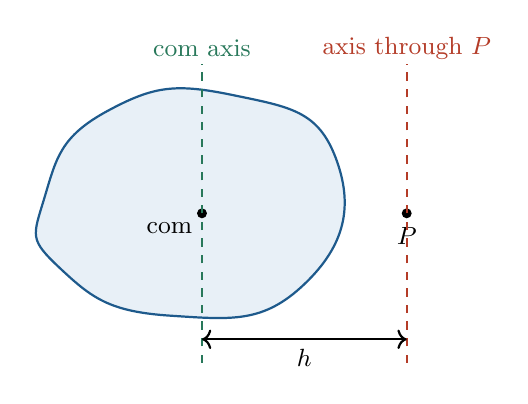
\begin{tikzpicture}[scale=1.0]
  \draw[thick,seccolor,fill=lightfill] plot[smooth cycle,tension=0.9]
    coordinates {(-2,0.2)(-1.2,1.3)(0.4,1.5)(1.7,0.7)(1.3,-0.9)(-0.4,-1.3)(-1.8,-0.7)};
  \fill (0,0) circle (1.8pt);
  \node[below left] at (0,0) {\small com};
  \draw[accent2,thick,dashed] (0,-1.9)--(0,1.9);
  \node[accent2] at (0,2.1) {\small com axis};
  \fill (2.6,0) circle (1.8pt);
  \node[below] at (2.6,-0.05) {\small $P$};
  \draw[accent,thick,dashed] (2.6,-1.9)--(2.6,1.9);
  \node[accent] at (2.6,2.1) {\small axis through $P$};
  \draw[<->,thick] (0,-1.6)--(2.6,-1.6) node[midway,below]{\small $h$};
\end{tikzpicture}
\end{document}
